% !TeX root = statnicaEKT.tex
\part{BPC-DE1 - Digitální elektronika 1}
\begin{huge}
	Otázky:
	\newline
\end{huge}
\begin{enumerate}
	\item Otázka - Logická hradla. Postuláty a zákony Booleovy algebry. 
	\item Otázka - Klopné obvody. Typy, vlastnosti, zapojení a realizace. 
	\item Otázka - Čítače. Typy, vlastnosti, zapojení a realizace. 
\end{enumerate}
%%%%%%%%%%%%%%%%%%%%%%%%%%%%%%%%%%%%%%%%%%%%%%%%%%%%%
\chapter{Logické hradlá, postuláty a zákony Boolovej algebry}
%%%%%%%%%%%%%%%%%%%%%%%%%%%%%%%%%%%%%%%%%%%%%%%%%%%%%

\section{Čo sú logické hradlá?}

Digitálne obvody pracujú len s dvoma hodnotami: \textbf{0} (nízke napätie, ``nepravda'') a \textbf{1} (vysoké napätie, ``pravda''). \textbf{Logické hradlo} je najjednoduchší stavebný blok -- elektronický obvod, ktorý vykoná jednu logickú operáciu a výsledok dá na výstup.

\begin{figure}[H]
    \centering
    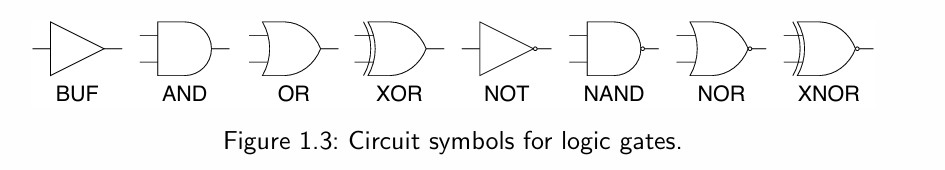
\includegraphics[width=0.85\textwidth]{Obrazky/Obrazky_DE1/fig_hradla_znacky.jpg}
    \caption{Schematické značky základných logických hradiel. Zľava: BUF (sledovač -- kopíruje vstup na výstup), AND (logický súčin), OR (logický súčet), XOR (exkluzívny súčet), NOT (invertor), NAND, NOR a XNOR. \textbf{Krúžok na výstupe vždy znamená negáciu.}}
    \label{fig:hradla_znacky}
\end{figure}

\section{Základné logické hradlá}

\subsection{AND -- logický súčin (``A zároveň'')}

AND hovorí: výstup je 1, len keď sú \textbf{oba} vstupy 1. Ako dva spínače zapojené za sebou -- prúd tečie, len keď sú zavreté oba.

\begin{minipage}{0.52\textwidth}
Výstup $y = a \cdot b$ je 1 iba ak $a=1$ \textbf{a zároveň} $b=1$.
\end{minipage}
\hfill
\begin{minipage}{0.44\textwidth}
\begin{center}
\begin{tabular}{cc|c}
\toprule
$a$ & $b$ & $y$ \\
\midrule
0 & 0 & 0 \\
0 & 1 & 0 \\
1 & 0 & 0 \\
1 & 1 & \textbf{1} \\
\bottomrule
\end{tabular}
\end{center}
\end{minipage}

\subsection{OR -- logický súčet (``alebo'')}

OR hovorí: výstup je 1, keď je aspoň jeden vstup 1. Ako dva spínače zapojené paralelne -- stačí zavrieť jeden.

\begin{minipage}{0.52\textwidth}
Výstup $y = a + b$ je 1 ak $a=1$ \textbf{alebo} $b=1$ (alebo oboje).
\end{minipage}
\hfill
\begin{minipage}{0.44\textwidth}
\begin{center}
\begin{tabular}{cc|c}
\toprule
$a$ & $b$ & $y$ \\
\midrule
0 & 0 & 0 \\
0 & 1 & \textbf{1} \\
1 & 0 & \textbf{1} \\
1 & 1 & \textbf{1} \\
\bottomrule
\end{tabular}
\end{center}
\end{minipage}

\subsection{NOT -- invertor (negácia)}

NOT obráti hodnotu: z 0 urobí 1 a z 1 urobí 0. Ako prepínač ``zapnuté/vypnuté''.

\subsection{XOR -- exkluzívny súčet (``jeden alebo druhý, ale nie obaja'')}

XOR hovorí: výstup je 1, ak sa vstupy \textbf{líšia}. Praktické využitie: detekcia rozdielu, sčítavanie bitov.

\begin{minipage}{0.52\textwidth}
Výstup $y = a \oplus b$ je 1, ak sú vstupy \textbf{rôzne}.
\end{minipage}
\hfill
\begin{minipage}{0.44\textwidth}
\begin{center}
\begin{tabular}{cc|c}
\toprule
$a$ & $b$ & $y$ \\
\midrule
0 & 0 & 0 \\
0 & 1 & \textbf{1} \\
1 & 0 & \textbf{1} \\
1 & 1 & 0 \\
\bottomrule
\end{tabular}
\end{center}
\end{minipage}

\subsection{NAND a NOR -- univerzálne hradlá}

NAND = AND s negovaným výstupom. NOR = OR s negovaným výstupom.

Prečo sú také dôležité? Sú to \textbf{univerzálne hradlá} -- z jedného typu (len z NANDov alebo len z NORov) možno zostrojiť \textit{akúkoľvek} logickú funkciu, teda aj AND, OR alebo NOT. V praxi sa celé procesory vyrábajú výhradne z NAND hradiel -- sú najjednoduchšie na výrobu v CMOS technológii.

\textbf{NAND ako NOT:} stačí spojiť oba vstupy dokopy: NAND($a$, $a$) = NOT($a$). Dve hradlá za sebou dajú AND.

\section{Boolova algebra -- pravidlá pre prácu s logickými výrazmi}

Boolova algebra je sada matematických pravidiel, ktoré popisujú správanie logických premenných. Umožňuje \textbf{zjednodušovať zložité výrazy} -- a tým zjednodušovať a šetriť hradlá v obvode.

\textbf{Vplyv konštánt -- čo sa stane, keď na vstup privedieme pevnú 0 alebo 1:}
\begin{center}
\begin{tabular}{ll}
$0 + a = a$ & OR s nulou: nula nič nepridá, výsledok závisí len na $a$ \\
$1 + a = 1$ & OR s jednotkou: jednotka vždy vyhrá, výsledok je vždy 1 \\
$1 \cdot a = a$ & AND s jednotkou: jednotka nič nezmení \\
$0 \cdot a = 0$ & AND s nulou: nula vždy vyhrá, výsledok je vždy 0 \\
$a + a = a$ & OR sám so sebou: nič nové \\
$a \cdot a = a$ & AND sám so sebou: nič nové \\
\end{tabular}
\end{center}

\textbf{Negácia:}
\begin{center}
\begin{tabular}{ll}
$a + \bar{a} = 1$ & premenná OR jej opak: vždy jeden z nich je 1, výsledok vždy 1 \\
$a \cdot \bar{a} = 0$ & premenná AND jej opak: nemôžu byť obe 1, výsledok vždy 0 \\
$\bar{\bar{a}} = a$ & dvojitá negácia sa ruší \\
\end{tabular}
\end{center}

\textbf{Komutatívnosť} -- na poradí nezáleží: $a + b = b + a$. Rovnako ako pri sčítavaní čísel.

\textbf{Asociatívnosť} -- závorky možno preusporiadať: $(a + b) + c = a + (b + c)$.

\textbf{Distributívnosť} -- roznásobovanie závoriek: $a \cdot (b + c) = a\cdot b + a\cdot c$.

\textbf{Absorpcia (pohltenie)} -- zjednodušenie, ktoré nie je na prvý pohľad zrejmé: $a + a \cdot b = a$. Prečo? Ak $a=1$, je výsledok 1 bez ohľadu na $b$. Ak $a=0$, potom $a \cdot b = 0$ tiež, výsledok je 0. Výsledok závisí len na $a$ -- $b$ je zbytočné.

\section{De Morganove zákony -- najdôležitejšie pravidlá}

De Morganove zákony hovoria, ako ``pretlačiť negáciu dovnútra'' výrazu. Sú kľúčové pre zjednodušovanie obvodov a pre pochopenie, prečo NAND a NOR sú ekvivalentné s inými kombináciami hradiel.

\medskip
\textbf{Zákon 1:} $\overline{a \cdot b} = \bar{a} + \bar{b}$\quad (NAND = OR s negovanými vstupmi)

Slovne: ``Nie je pravda, že A aj B'' = ``Buď nie je A, alebo nie je B.''

Príklad zo života: ``Nezatvoril som dvere \textbf{a} okno'' = ``Buď som nezatvoril dvere, \textbf{alebo} som nezatvoril okno.''

\medskip
\textbf{Zákon 2:} $\overline{a + b} = \bar{a} \cdot \bar{b}$\quad (NOR = AND s negovanými vstupmi)

Slovne: ``Nie je pravda, že A alebo B'' = ``Ani A, ani B.''

Príklad zo života: ``Nesvieti lampa \textbf{ani} televízor'' = ``Nesvieti lampa \textbf{a zároveň} nesvieti televízor.''

\medskip
\textbf{Praktický dôsledok:} Každý AND možno nahradiť NORom s negovanými vstupmi a naopak. To znamená, že celý obvod možno realizovať len z jedného typu hradla.

\textbf{Princíp duality:} Každý platný výraz Boolovej algebry zostane platný, keď vymeníme AND$\leftrightarrow$OR a $0\leftrightarrow 1$ všade. De Morganove zákony sú presne takým párom.

\section{Minimalizácia logických funkcií}

Každú logickú funkciu možno zapísať ako \textbf{tabuľku pravdivosti} -- pre každú kombináciu vstupov je uvedený výstup. Z tabuľky zostrojíme obvod, ale ten býva zbytočne zložitý. Minimalizácia hľadá ekvivalentný, ale jednoduchší výraz.

\textbf{SoP (Sum of Products)} -- súčet súčinov: pre každý riadok kde je výstup 1 napíšeme súčin všetkých vstupov (mintermový term), potom ich sčítame (OR). Priamočiare, ale výraz nemusí byť najjednoduchší.

\textbf{PoS (Product of Sums)} -- súčin súčtov: podobný postup, ale vychádzame z riadkov kde je výstup 0.

\textbf{Karnaughova mapa (K-mapa):} grafická metóda zjednodušovania, praktická pre funkcie do 4 premenných. Tabuľka pravdivosti sa prepíše do špeciálnej mriežky, kde susedné políčka sa líšia práve v jednom bite. Skupiny susedných jednotiek zodpovedajú zjednodušeným súčinom -- čím väčšia skupina ($1, 2, 4, 8$ políčok), tým jednoduchší výsledný výraz.

\newpage

%%%%%%%%%%%%%%%%%%%%%%%%%%%%%%%%%%%%%%%%%%%%%%%%%%%%%
\chapter{Klopné obvody -- typy, vlastnosti, zapojenie a realizácia}
%%%%%%%%%%%%%%%%%%%%%%%%%%%%%%%%%%%%%%%%%%%%%%%%%%%%%

\section{Prečo potrebujeme klopné obvody?}

Logické hradlá sú \textbf{kombinačné} -- výstup závisí len na aktuálnych vstupoch, bez pamäte. Ale procesor potrebuje \textbf{pamätať si} hodnoty -- výsledky výpočtov, aktuálny stav systému, obsah registrov. Na to slúžia \textbf{klopné obvody} -- majú dva stabilné stavy (0 a 1) a samy si udržia svoj stav, kým ho niekto nezmení.

Analógia: klopný obvod je ako svetelný vypínač -- zostane v stave ``zapnuté'' alebo ``vypnuté'', kým ho neprepnete.

\textbf{Dva základné typy:}
\begin{itemize}
    \item \textbf{Latch (asynchrónny):} reaguje okamžite na \textbf{úroveň} riadiaceho signálu. Kým je EN aktívny, vstup prechádza priamo na výstup (``transparentný'').
    \item \textbf{Flip-flop (synchrónny):} reaguje presne na \textbf{hranu} hodinového signálu (prechod 0$\rightarrow$1 alebo 1$\rightarrow$0). Mimo hrany je vstup zmrazený -- výstup sa nemení.
\end{itemize}

\section{S-R Latch -- najjednoduchší pamäťový prvok}

S-R latch má dva vstupy: \textbf{S} (Set -- nastav $Q$ na 1) a \textbf{R} (Reset -- nastav $Q$ na 0). Výstupy $Q$ a $\bar{Q}$ sú vždy vzájomne opačné (jeden je 0, druhý 1).

\subsection{Realizácia pomocou NOR hradiel}

\begin{figure}[H]
    \centering
    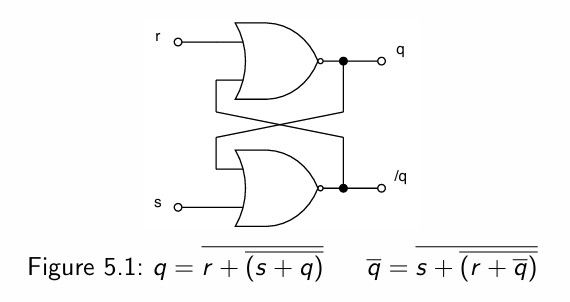
\includegraphics[width=0.45\textwidth]{Obrazky/Obrazky_DE1/fig_sr_latch_nor.jpg}
    \caption{S-R latch z dvoch NOR hradiel. Kľúčom je \textbf{spätná väzba} -- výstup každého hradla je privedený na vstup druhého. Vďaka tomu sa obvod ``udrží'' v nastavenom stave aj po uvoľnení vstupu -- to je princíp pamäte.}
    \label{fig:sr_latch_nor}
\end{figure}

Ako si obvod pamätá: nastavíme $S=1$ a $Q$ sa prepne na 1. Spätná väzba potom zabezpečí, že $Q=1$ drží výstup druhého NOR hradla na 0, a to zase drží $Q=1$ -- slučka sa ``uzamkla''. Po uvoľnení $S$ zostane $Q=1$.

\begin{center}
\begin{tabular}{cc|cc|l}
\toprule
$S$ & $R$ & $Q$ & $\bar{Q}$ & Čo sa deje \\
\midrule
0 & 0 & $Q$ & $\bar{Q}$ & \textbf{Pamäť} -- stav sa nemení \\
1 & 0 & 1 & 0 & \textbf{Set} -- nastav $Q$ na 1 \\
0 & 1 & 0 & 1 & \textbf{Reset} -- nastav $Q$ na 0 \\
1 & 1 & ? & ? & \textbf{ZAKÁZANÉ!} -- výstupy nie sú opačné \\
\bottomrule
\end{tabular}
\end{center}

\begin{figure}[H]
    \centering
    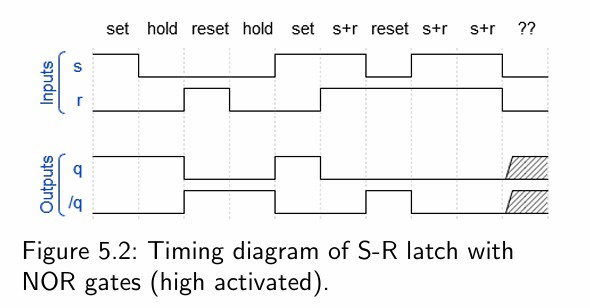
\includegraphics[width=0.55\textwidth]{Obrazky/Obrazky_DE1/fig_sr_latch_nor_timing.jpg}
    \caption{Časový diagram S-R latchu. $S=1$ prepne $Q$ na 1. $R=1$ vráti $Q$ na 0. Šrafovaná oblasť je zakázaný stav ($S=R=1$) -- pri návrate z tohto stavu nevieme, v akom stave sa obvod ustáli (\textbf{metastabilita}).}
    \label{fig:sr_latch_nor_timing}
\end{figure}

\textbf{Zakázaný stav a metastabilita:} Ak sú oba vstupy $S=R=1$ a potom oba naraz prejdú na 0, obvod nevie, do akého stavu skočiť. Ocitne sa v \textbf{metastabilnom stave} -- výstup osciluje alebo sa ustáli na neurčitej hodnote po dobu desiatok nanosekúnd. To môže pokaziť funkciu celého systému.

\subsection{Realizácia pomocou NAND hradiel}

Funguje rovnako, ale aktívna úroveň je opačná -- obvod reaguje na \textbf{nízku} (log. 0) úroveň vstupov $\bar{S}$ a $\bar{R}$.

\begin{figure}[H]
    \centering
    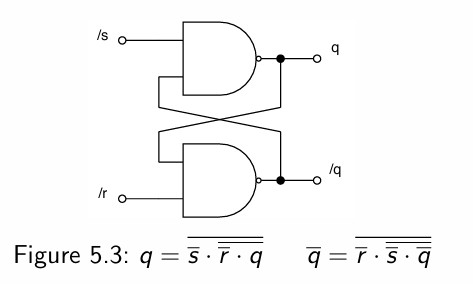
\includegraphics[width=0.45\textwidth]{Obrazky/Obrazky_DE1/fig_sr_latch_nand.jpg}
    \caption{S-R latch z dvoch NAND hradiel. Oproti NOR verzii sú vstupné úrovne invertované -- pokojový stav (pamäť) je $\bar{S}=\bar{R}=1$, zakázaný stav je $\bar{S}=\bar{R}=0$.}
    \label{fig:sr_latch_nand}
\end{figure}

\section{Gated S-R Latch -- pridáme povoľovací vstup}

Základný S-R latch reaguje ihneď -- kedykoľvek sa zmení $S$ alebo $R$, výstup okamžite reaguje. V praxi potrebujeme riadiť, \textbf{kedy} smie obvod reagovať. Gated latch pridáva vstup \textbf{EN (Enable)}:

\begin{itemize}
    \item $EN = 1$: obvod je ``odomknutý'' -- sleduje vstupy normálne
    \item $EN = 0$: obvod je ``zamknutý'' -- ignoruje vstupy, drží posledný stav
\end{itemize}

\begin{figure}[H]
    \centering
    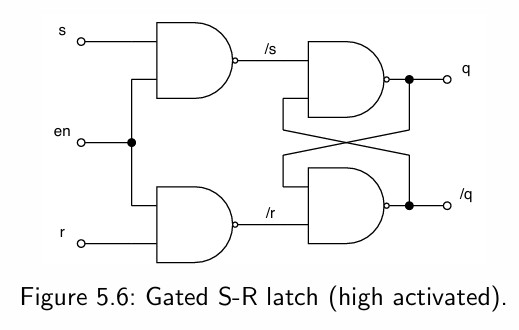
\includegraphics[width=0.50\textwidth]{Obrazky/Obrazky_DE1/fig_gated_sr_latch.jpg}
    \caption{Gated S-R latch. Pridané AND hradlá fungujú ako ``brána'' -- prepustia $S$ a $R$ len vtedy, keď $EN=1$. Pri $EN=0$ sú oba vstupy AND hradiel nulové a vnútorný SR latch drží svoj stav.}
    \label{fig:gated_sr_latch}
\end{figure}

\begin{figure}[H]
    \centering
    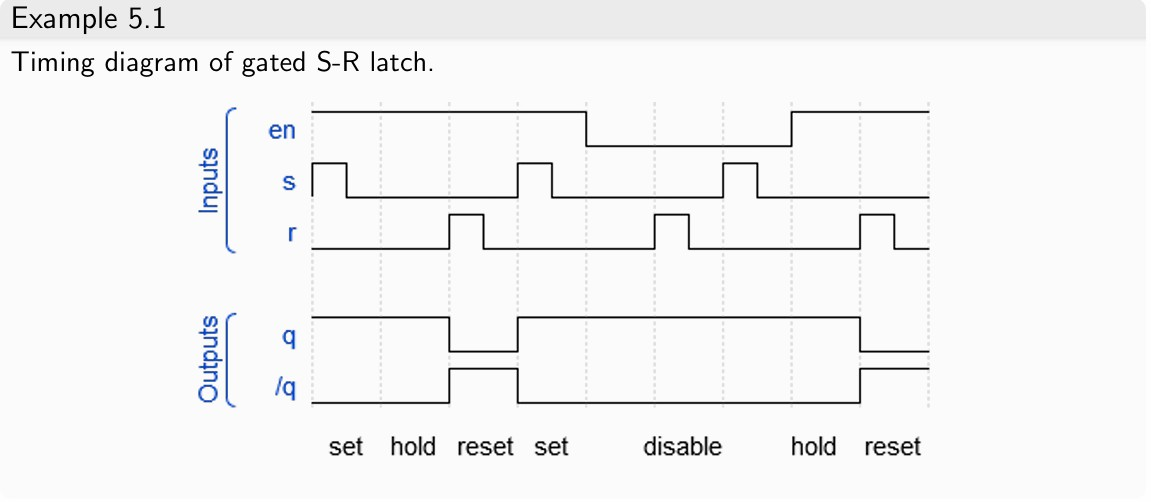
\includegraphics[width=0.60\textwidth]{Obrazky/Obrazky_DE1/fig_gated_sr_timing.jpg}
    \caption{Časový diagram Gated S-R latchu -- vidíme postupne štyri situácie: set (nastavenie), hold (udržanie), reset (vynulovanie) a disable ($EN=0$, obvod ignoruje vstupy a drží posledný stav).}
    \label{fig:gated_sr_timing}
\end{figure}

\section{D Latch -- transparentný latch}

S-R latch má zakázaný stav ($S=R=1$). Ako ho odstrániť? Jednoducho: pridáme invertor tak, aby $R$ bolo vždy opakom $S$. Tým $S$ a $R$ nikdy nemôžu byť oba 1 naraz. Vstup premenujeme na \textbf{D (Data)}.

\begin{figure}[H]
    \centering
    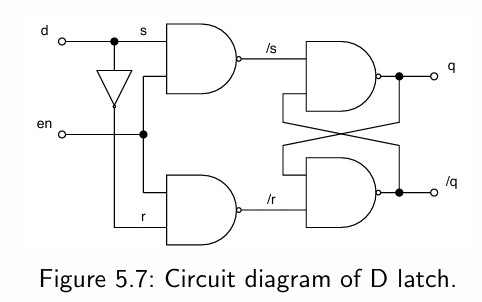
\includegraphics[width=0.50\textwidth]{Obrazky/Obrazky_DE1/fig_d_latch.jpg}
    \caption{D latch. Invertor zaručuje $R = \bar{D}$ -- zakázaný stav SR latchu nemôže nastať. Pri $EN=1$ výstup $Q$ okamžite sleduje vstup $D$ (``transparentný'' režim). Na zostupnej hrane EN sa aktuálna hodnota $D$ uzamkne.}
    \label{fig:d_latch}
\end{figure}

\begin{figure}[H]
    \centering
    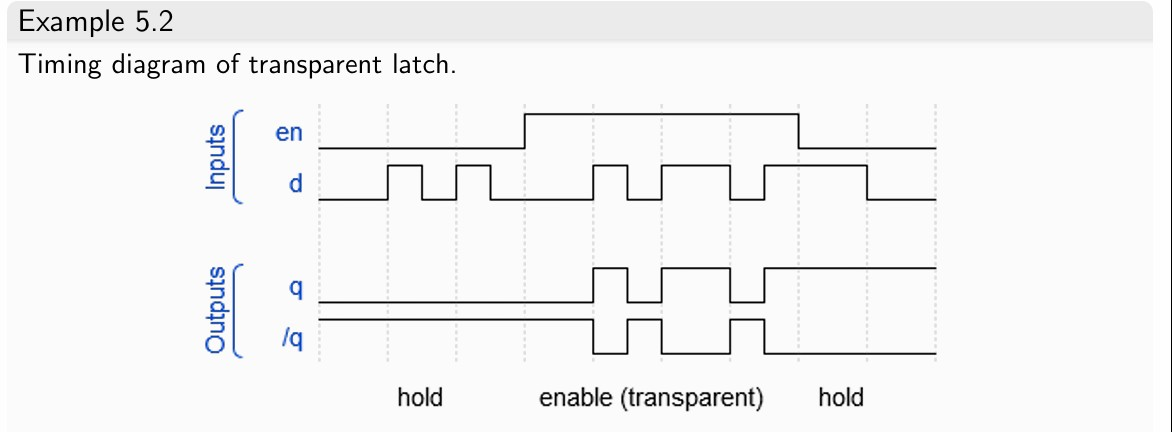
\includegraphics[width=0.60\textwidth]{Obrazky/Obrazky_DE1/fig_d_latch_timing.jpg}
    \caption{Časový diagram D latchu. Pri $EN=1$ výstup $Q$ okamžite kopíruje vstup $D$. Na zostupnej hrane $EN$ sa aktuálna hodnota ``uzamkne'' a $Q$ ju drží aj po deaktivácii -- to je princíp latchu.}
    \label{fig:d_latch_timing}
\end{figure}

\textbf{Problém D latchu:} ak sa $D$ zmení v čase, keď $EN=1$, okamžite to prejde na výstup. V synchrónnych systémoch chceme, aby ku zmene došlo \textbf{presne na hrane hodín} -- nie kedykoľvek. To rieši flip-flop.

\section{D Flip-flop -- reaguje len na hranu hodín}

D flip-flop rieši problém D latchu tým, že \textbf{dva D latche zapojí za sebou} s opačnými hodinami -- tzv. \textbf{Master-Slave štruktúra}.

\begin{figure}[H]
    \centering
    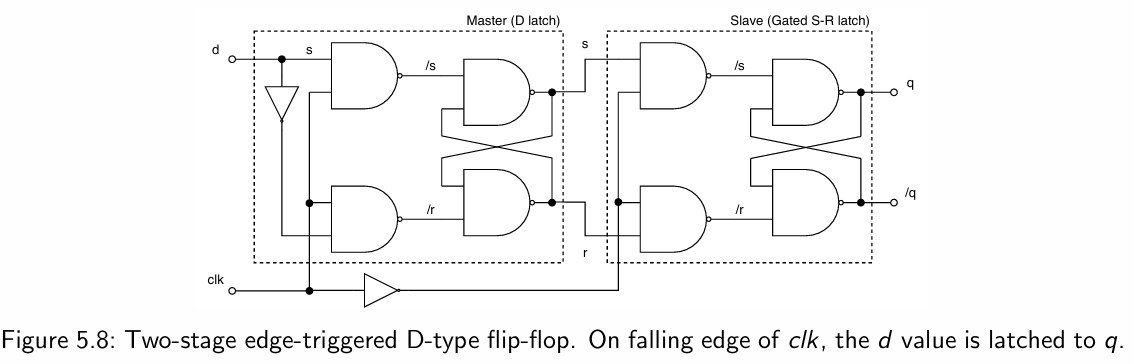
\includegraphics[width=0.80\textwidth]{Obrazky/Obrazky_DE1/fig_d_ff_master_slave.jpg}
    \caption{Master-Slave D flip-flop z dvoch latchov. Master (vľavo) sa otvorí pri $CLK=1$ a zachytí $D$. Slave (vpravo) sa otvorí pri $CLK=0$ (invertované hodiny) a prepustí hodnotu na výstup $Q$. Nikdy nie sú oba otvorené naraz -- výstup sa zmení len raz za periódu, presne na hrane CLK.}
    \label{fig:d_ff_master_slave}
\end{figure}

\textbf{Ako to funguje krok po kroku:}
\begin{enumerate}
    \item $CLK$ prejde na 1 $\Rightarrow$ Master sa otvorí a zachytí aktuálne $D$; Slave je zamknutý
    \item $CLK$ prejde na 0 $\Rightarrow$ Master sa uzavrie (uzamkne zachytenú hodnotu); Slave sa otvorí a prepustí túto hodnotu na výstup $Q$
\end{enumerate}

Výsledok: $Q$ sa zmení vždy presne na \textbf{zostupnej hrane CLK} -- nie skôr, nie neskôr. Charakteristická rovnica: $Q_{n+1} = D$ (po hrane je výstup rovný vstupu pred hranou).

\begin{figure}[H]
    \centering
    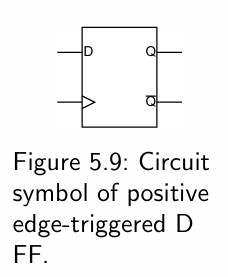
\includegraphics[width=0.22\textwidth]{Obrazky/Obrazky_DE1/fig_d_ff_symbol.jpg}
    \caption{Schematická značka D flip-flopu. Trojuholník na vstupe CLK znamená ``reaguje na hranu''. Verzia bez trojuholníka = latch (reaguje na úroveň).}
    \label{fig:d_ff_symbol}
\end{figure}

\begin{figure}[H]
    \centering
    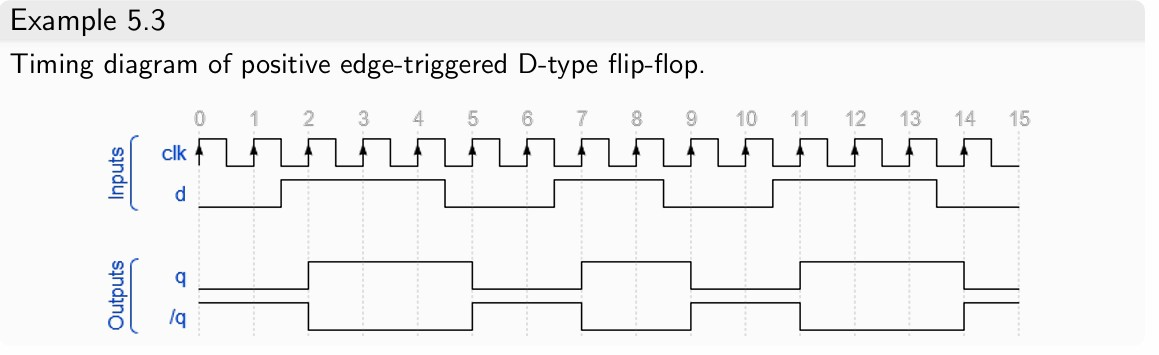
\includegraphics[width=0.75\textwidth]{Obrazky/Obrazky_DE1/fig_d_ff_timing.jpg}
    \caption{Časový diagram D flip-flopu s nábežnou hranou. $Q$ preberá hodnotu $D$ vždy len v okamžiku nábežnej hrany CLK ($\uparrow$). Medzi hranami zostáva $Q$ stabilné bez ohľadu na zmeny $D$.}
    \label{fig:d_ff_timing}
\end{figure}

\section{JK Flip-flop -- zakázaný stav sa stane užitočným}

JK flip-flop vychádza zo SR flip-flopu, ale zakázaný stav ($J=K=1$) mení na užitočnú funkciu: \textbf{Toggle} -- prehoď výstup na opačnú hodnotu. Dosiahne to spätnými väzbami z $Q$ a $\bar{Q}$ do vstupov.

\begin{figure}[H]
    \centering
    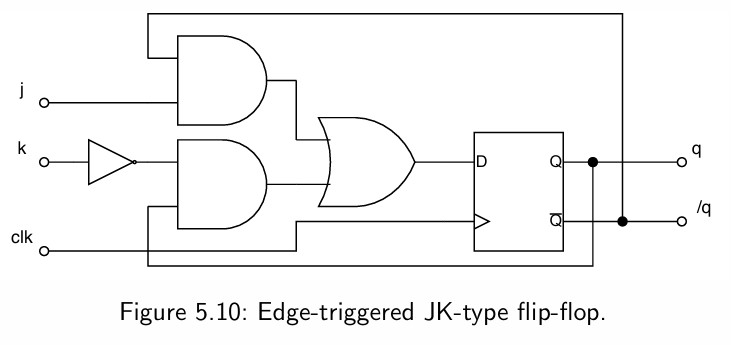
\includegraphics[width=0.70\textwidth]{Obrazky/Obrazky_DE1/fig_jk_ff.jpg}
    \caption{JK flip-flop. Spätné väzby z výstupov $Q$ a $\bar{Q}$ do vstupných AND hradiel zabránia zakázanému stavu -- kombinácia $J=K=1$ spôsobí toggle namiesto neurčitého stavu. Ak je $Q=1$, vstup cez AND pre $J$ je blokovaný hodnotou $\bar{Q}=0$, takže sa môže len resetovať (a naopak).}
    \label{fig:jk_ff}
\end{figure}

\begin{center}
\begin{tabular}{cc|c|l}
\toprule
$J$ & $K$ & $Q_{n+1}$ & Čo sa deje \\
\midrule
0 & 0 & $Q_n$       & \textbf{Pamäť} -- nič sa nemení \\
0 & 1 & 0           & \textbf{Reset} -- vynuluj \\
1 & 0 & 1           & \textbf{Set} -- nastav na 1 \\
1 & 1 & $\bar{Q}_n$ & \textbf{Toggle} -- prehoď! \\
\bottomrule
\end{tabular}
\end{center}

\begin{figure}[H]
    \centering
    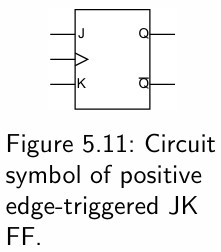
\includegraphics[width=0.22\textwidth]{Obrazky/Obrazky_DE1/fig_jk_ff_symbol.jpg}
    \caption{Schematická značka JK flip-flopu. $J$ zodpovedá Set, $K$ zodpovedá Reset -- navyše $J=K=1$ prehodí výstup.}
    \label{fig:jk_ff_symbol}
\end{figure}

\textbf{Excitačná tabuľka} -- aké $J$ a $K$ potrebujem, aby sa výstup prepol z $Q_n$ na $Q_{n+1}$? Potrebujeme ju pri návrhu sekvenčných obvodov (stavových automatov):

\begin{center}
\begin{tabular}{cc|cc}
\toprule
$Q_n$ & $Q_{n+1}$ & $J$ & $K$ \\
\midrule
0 & 0 & 0 & $\times$ (jedno čo) \\
0 & 1 & 1 & $\times$ \\
1 & 0 & $\times$ & 1 \\
1 & 1 & $\times$ & 0 \\
\bottomrule
\end{tabular}
\end{center}

\section{T Flip-flop -- delič frekvencie}

T flip-flop vznikne z JK flip-flopu jednoducho: spojíme oba vstupy $J$ a $K$ do jedného vstupu $T$. Má len dve funkcie:

\begin{center}
\begin{tabular}{c|c|l}
\toprule
$T$ & $Q_{n+1}$ & Čo sa deje \\
\midrule
0 & $Q_n$       & \textbf{Pamäť} -- drž stav \\
1 & $\bar{Q}_n$ & \textbf{Toggle} -- prehoď \\
\bottomrule
\end{tabular}
\end{center}

\begin{figure}[H]
    \centering
    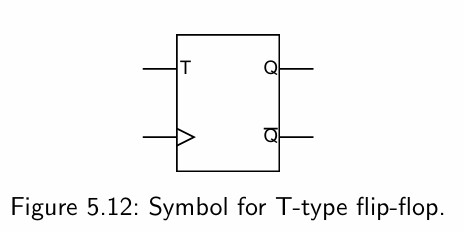
\includegraphics[width=0.22\textwidth]{Obrazky/Obrazky_DE1/fig_t_ff_symbol.jpg}
    \caption{Schematická značka T flip-flopu. Pri trvale $T=1$ sa výstup prehadzuje na každej hrane CLK -- výstupná frekvencia je presne \textbf{polovičná} oproti CLK.}
    \label{fig:t_ff_symbol}
\end{figure}

\textbf{Kľúčová vlastnosť:} T flip-flop s $T=1$ delí frekvenciu hodinového signálu presne dvoma. Kaskáda $n$ T flip-flopov delí frekvenciu $2^n$-krát. To je základ binárnych čítačov.

\section{Časové parametre -- kedy musí byť vstup stabilný?}

Flip-flop zachytí hodnotu $D$ presne na hrane CLK. Ale elektronické obvody nie sú ideálne -- potrebujú čas na spracovanie. Preto musí byť $D$ stabilné po určitú dobu \textit{okolo} hrany CLK.

\begin{figure}[H]
    \centering
    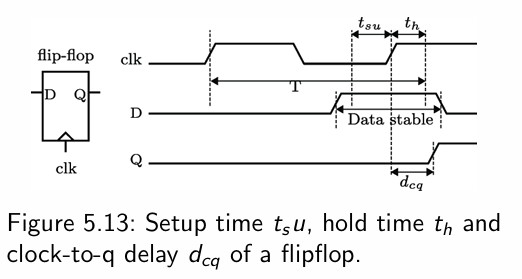
\includegraphics[width=0.80\textwidth]{Obrazky/Obrazky_DE1/fig_setup_hold.jpg}
    \caption{Časové parametre flip-flopu. \textbf{Setup time $t_{su}$}: $D$ musí byť stabilné najmenej $t_{su}$ \textit{pred} hranou CLK. \textbf{Hold time $t_h$}: $D$ musí zostať stabilné najmenej $t_h$ \textit{po} hrane CLK. \textbf{Clock-to-Q $d_{cq}$}: výstup $Q$ sa zmení až za $d_{cq}$ po hrane -- flip-flop potrebuje čas na ``prepnutie''.}
    \label{fig:setup_hold}
\end{figure}

\textbf{Čo sa stane pri porušení?} Flip-flop sa dostane do \textbf{metastabilného stavu} -- nezachytí ani 0 ani 1, výstup sa chvíľu nevyrovná a spôsobuje chyby v celom systéme.

\textbf{Maximálna hodinová frekvencia} -- hodiny môžu tikať len tak rýchlo, ako rýchlo sa stihne propagovať signál z výstupu cez kombinačnú logiku späť na vstup. Platí: $f_{max} = 1 / (d_{cq} + t_{comb} + t_{su})$.

\section{Posuvné registre}

Posuvný register je rad D flip-flopov zapojených za sebou -- výstup $Q$ jedného ide na vstup $D$ ďalšieho, všetky na spoločnom CLK. Pri každom takte sa dáta posunú o jeden krok doprava.

Použitie:
\begin{itemize}
    \item \textbf{SIPO} (Serial In, Parallel Out): prijať dáta sériovo (bit po bite) a čítať ich naraz paralelne -- napríklad čítanie dát zo SPI obvodu
    \item \textbf{PISO} (Parallel In, Serial Out): prijať dáta paralelne a odosielať ich sériovo
    \item Oneskorenie signálu o presne $n$ taktov
\end{itemize}

\newpage

%%%%%%%%%%%%%%%%%%%%%%%%%%%%%%%%%%%%%%%%%%%%%%%%%%%%%
\chapter{Čítače -- typy, vlastnosti, zapojenie a realizácia}
%%%%%%%%%%%%%%%%%%%%%%%%%%%%%%%%%%%%%%%%%%%%%%%%%%%%%

\section{Čo je čítač a na čo slúži?}

Čítač je sekvenčný obvod, ktorý \textbf{počíta hodinové impulzy}. Jeho výstup je binárne číslo, ktoré sa s každým taktom zvyšuje (alebo znižuje). Čítače sú základom časovačov, frekvenčných deličov, adresovania pamäte a mnohých ďalších aplikácií.

Kľúčové pojmy:
\begin{itemize}
    \item $n$ flip-flopov $\Rightarrow$ maximálne $2^n$ rôznych stavov
    \item \textbf{Modulus (MOD)}: koľko stavov čítač prejde pred návratom na začiatok. MOD-8 prejde stavmi 0, 1, 2, \ldots, 7 a vráti sa.
\end{itemize}

\section{Asynchrónny čítač (Ripple counter)}

\textbf{Myšlienka:} T flip-flop s $T=1$ delí frekvenciu dvoma -- výstup sa prehadzuje každý takt. Zapojme za sebou viac T flip-flopov, kde každý taktuje ten nasledujúci. Každý stupeň delí frekvenciu predchádzajúceho dvoma a výsledkom je binárny čítač!

\begin{figure}[H]
    \centering
    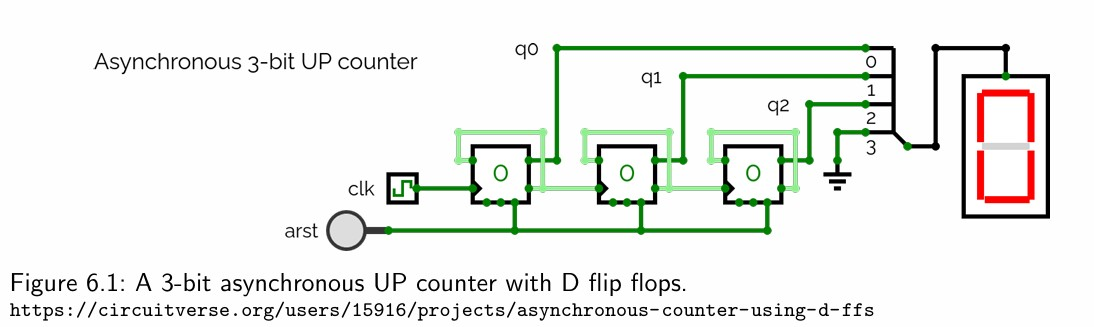
\includegraphics[width=0.75\textwidth]{Obrazky/Obrazky_DE1/fig_async_counter.jpg}
    \caption{3-bitový asynchrónny UP čítač. Každý D flip-flop má $D$ spojené s $\bar{Q}$ (toggle). Výstup $\bar{Q}$ každého stupňa taktuje stupeň nasledujúci. $Q_0$ sa mení každý takt, $Q_1$ každý druhý, $Q_2$ každý štvrtý -- dokopy tvoria binárny čítač 0--7.}
    \label{fig:async_counter}
\end{figure}

\textbf{Výhoda:} extrémne jednoduché zapojenie, žiadna kombinačná logika.

\begin{figure}[H]
    \centering
    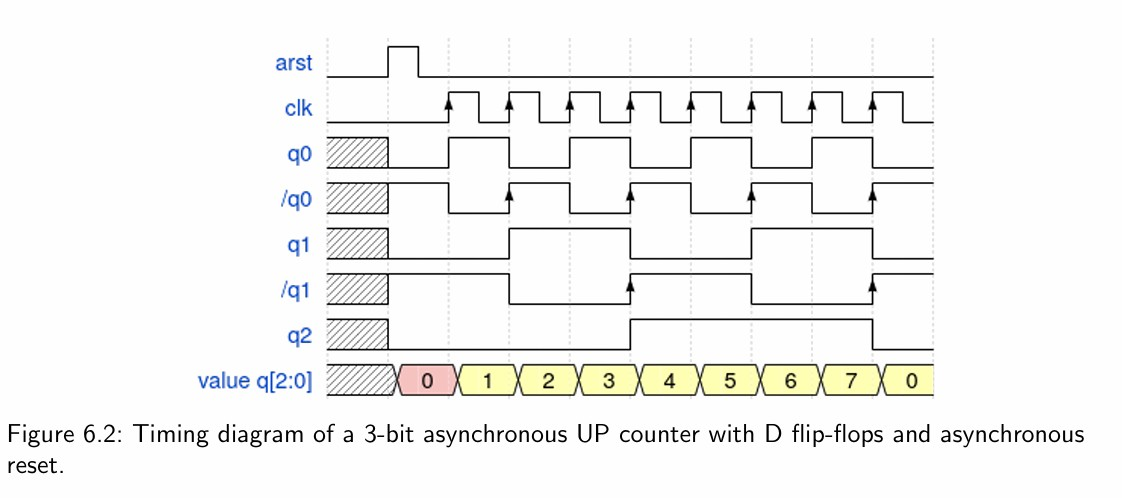
\includegraphics[width=0.75\textwidth]{Obrazky/Obrazky_DE1/fig_async_counter_timing.jpg}
    \caption{Časový diagram asynchrónneho čítača. Pri prechode 3$\rightarrow$4 (binárne $011 \to 100$) sa menia všetky tri bity -- ale nie naraz. Vidíme krátke falošné (glitch) hodnoty (010, 000) kým sa všetko ustáli. To je hlavná nevýhoda asynchrónneho čítača.}
    \label{fig:async_counter_timing}
\end{figure}

\subsection{Ripple efekt -- hlavná nevýhoda}

Prečo sa volá ``ripple'' (vlna)? Pretože zmena sa šíri ako vlna -- prvý flip-flop sa prepne, potom druhý, potom tretí\ldots Každý pridá svoje oneskorenie $t_{FF}$.

\textbf{Pri prechode 011 $\rightarrow$ 100} sa menia všetky tri bity, ale postupne -- v medziobdobí sa na výstupe krátko objavia \textbf{falošné (glitch) hodnoty}. To spôsobuje problémy, ak výstup čítača riadi iné obvody.

\textbf{Maximálna frekvencia} klesá s počtom bitov: s každým pridaným flip-flopom narastá oneskorenie o $t_{FF}$, teda $f_{max} = 1/(n \cdot t_{FF} + t_{su})$.

\section{Synchrónny čítač}

\textbf{Riešenie ripple efektu:} zapojíme všetky flip-flopy na \textbf{spoločný CLK} signál. Všetky sa prepnú \textbf{v rovnaký okamih} -- glitche zmiznú.

Nevýhoda: musíme pridať kombinačnú logiku, ktorá každému flip-flopu povie, či sa má v tomto takte prepnúť alebo nie.

\begin{figure}[H]
    \centering
    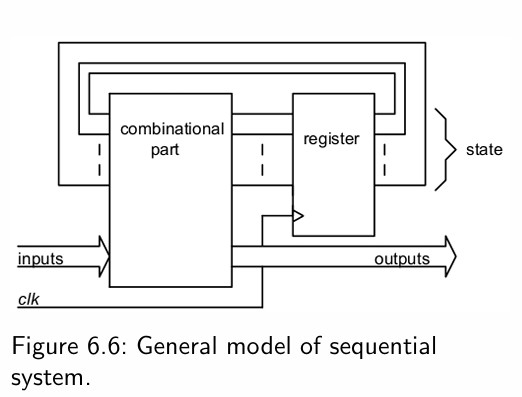
\includegraphics[width=0.50\textwidth]{Obrazky/Obrazky_DE1/fig_sync_model.jpg}
    \caption{Všeobecný model synchrónneho sekvenčného systému. Kombinačná logika na základe aktuálneho stavu vypočíta, čo bude v nasledujúcom takte. Register (flip-flopy) si všetko zapamätá na hrane CLK. Spätná väzba uzatvára slučku.}
    \label{fig:sync_model}
\end{figure}

\textbf{Pravidlo pre T flip-flopy:} bit $Q_i$ sa má prepnúť (toggle), iba keď \textbf{všetky nižšie bity sú jednotky} -- vtedy pretekajú a spôsobia prenos do vyššieho bitu.

\begin{itemize}
    \item $Q_0$: prepne sa vždy ($T_0 = 1$)
    \item $Q_1$: prepne sa, keď $Q_0 = 1$
    \item $Q_2$: prepne sa, keď $Q_1 = 1$ a $Q_0 = 1$
\end{itemize}

\textbf{Dva typy propagácie prenosu:}
\begin{itemize}
    \item \textbf{Parallel carry}: jedno veľké AND hradlo sleduje všetky nižšie bity naraz -- rýchle, ale AND hradlo rastie s každým bitom
    \item \textbf{Ripple carry}: prenos sa šíri postupne cez kaskádu 2-vstupových AND hradiel -- úspornejšie, ale pomalšie
\end{itemize}

\section{LFSR -- pseudonáhodný generátor}

\textbf{LFSR (Linear Feedback Shift Register)} je posuvný register, ktorého vstup je XOR kombinácia vybraných výstupov (tzv. ``taps''). Výsledkom je \textbf{pseudonáhodná sekvencia} -- postupnosť, ktorá vyzerá náhodne, ale je deterministická a opakuje sa.

\begin{figure}[H]
    \centering
    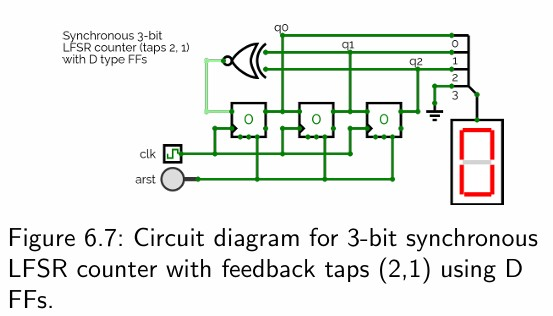
\includegraphics[width=0.65\textwidth]{Obrazky/Obrazky_DE1/fig_lfsr.jpg}
    \caption{3-bitový LFSR. Dáta sa posúvajú doprava. Spätná väzba z $Q_2$ a $Q_1$ cez XOR generuje nový bit na vstupe $D_0$. Stav $000$ sa nikdy neobjaví (XOR samých núl dá nulu -- zacyklenie). Sekvencia prechádza $2^3 - 1 = 7$ rôznymi stavmi.}
    \label{fig:lfsr}
\end{figure}

\textbf{Prečo $2^n - 1$ a nie $2^n$ stavov?} Stav samých núl je ``mŕtvy'' -- XOR samých núl dá opäť nulu, LFSR by sa nikdy nedostal z tohto stavu. Preto ho preskočíme (alebo použijeme XNOR a preskočíme stav samých jednotiek).

\textbf{Použitie:} generovanie testovacích sekvencií, kryptografia (stream ciphers), prenosové protokoly (scrambling), Wi-Fi pseudonáhodné sekvencie.

\section{Porovnanie: asynchrónny vs. synchrónny čítač}

\begin{center}
\begin{tabular}{lll}
\toprule
\textbf{Vlastnosť} & \textbf{Asynchrónny} & \textbf{Synchrónny} \\
\midrule
Taktovanie flip-flopov & Každý iným signálom   & Všetky rovnakým CLK \\
Glitche na výstupe     & Áno (ripple efekt)    & Nie \\
Kombinačná logika      & Žiadna                & AND hradlá pre prenos \\
Maximálna frekvencia   & Klesá s počtom bitov  & Nezávisí na počte bitov \\
Zložitosť návrhu       & Veľmi jednoduchý      & Stredne zložitý \\
Použitie               & Delič frekvencie, RTC & Procesory, FPGA, DSP \\
\bottomrule
\end{tabular}
\end{center}